\section{Events}
	\subsubsection{Qualifying competitions}
		\begin{enumerate}
			\item Sochi. Sochi was the first time the team participated in a comptetition. There, our team felt the spirit of FCS comptetion and noble professionalism for the first time. We got work experience all day and all night, began to make acquaintance among the teams, and providing all possible help we could. The planning and organization were all very nice. The most memorable contact we made was with the American team Stuy Fission 310, with which we now keep in touch. As a result we won a place in the regional finals.
			\center{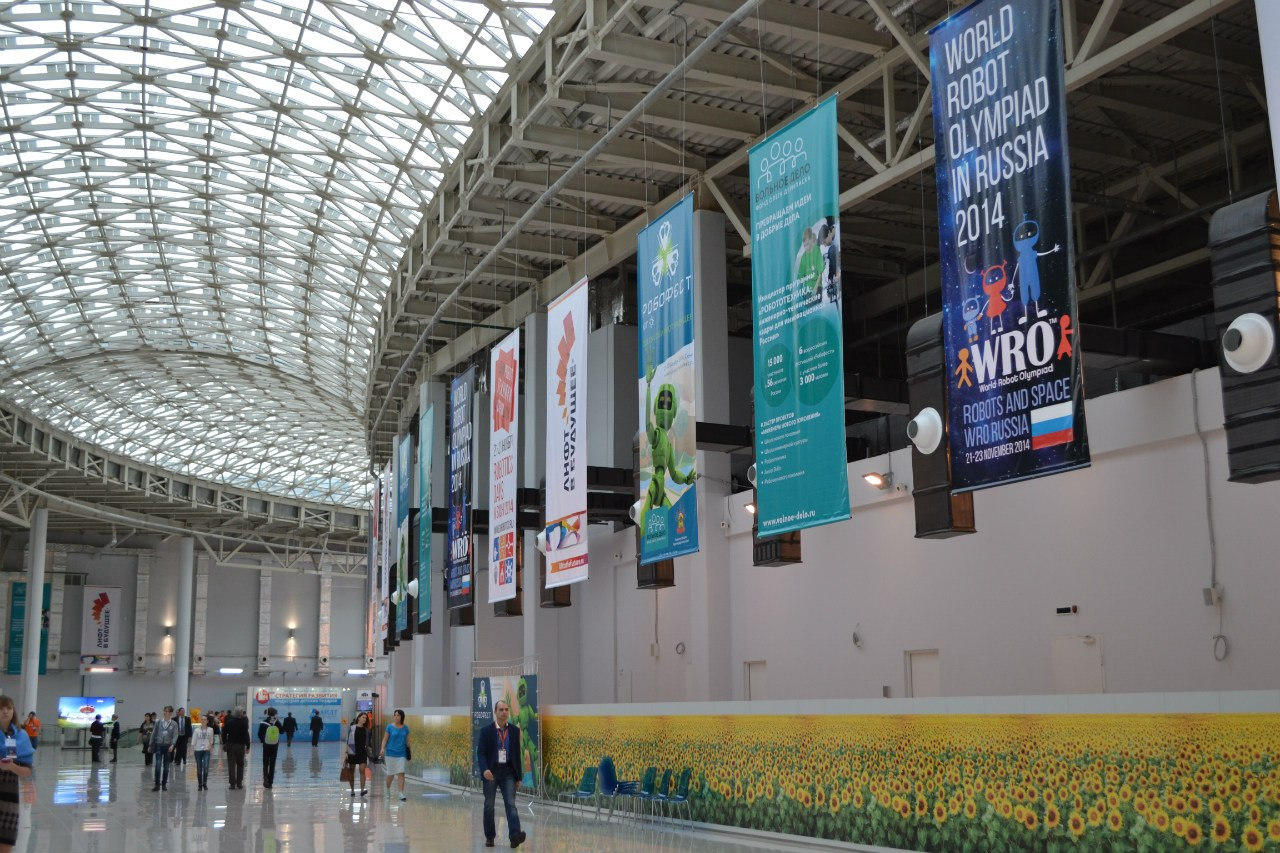
\includegraphics[scale=0.2]{days/Event/images/6}}\\
			\item Ryazan. Our first priority was to train on a real field. These competitions were quite small and quiet, all the teams communicated abundantly and shared ideas freely. We all felt comfortable there. The team helped to assemble and disassemble the field. As a result Participants of the alliance winner. 
			\center{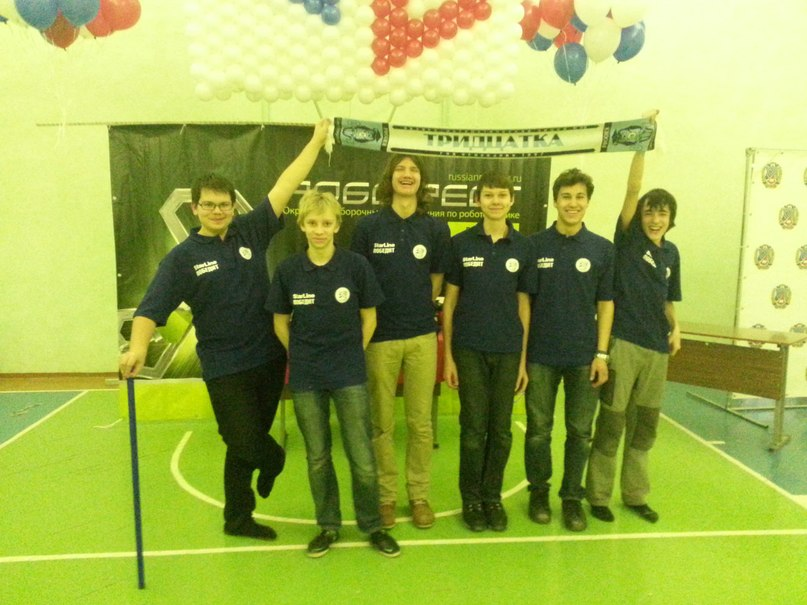
\includegraphics[scale=0.2]{days/Event/images/1}}\\	
			\item Perm. Dress rehearsal before the regional final. It was well organized event where we were able to practice in all aspects of the competition, including such important as the choice of Composes alliances finale.takzhe we strongly helped organizer with the technical part. As a result: the alliance of winners as well as first place in the general classification.
			\center{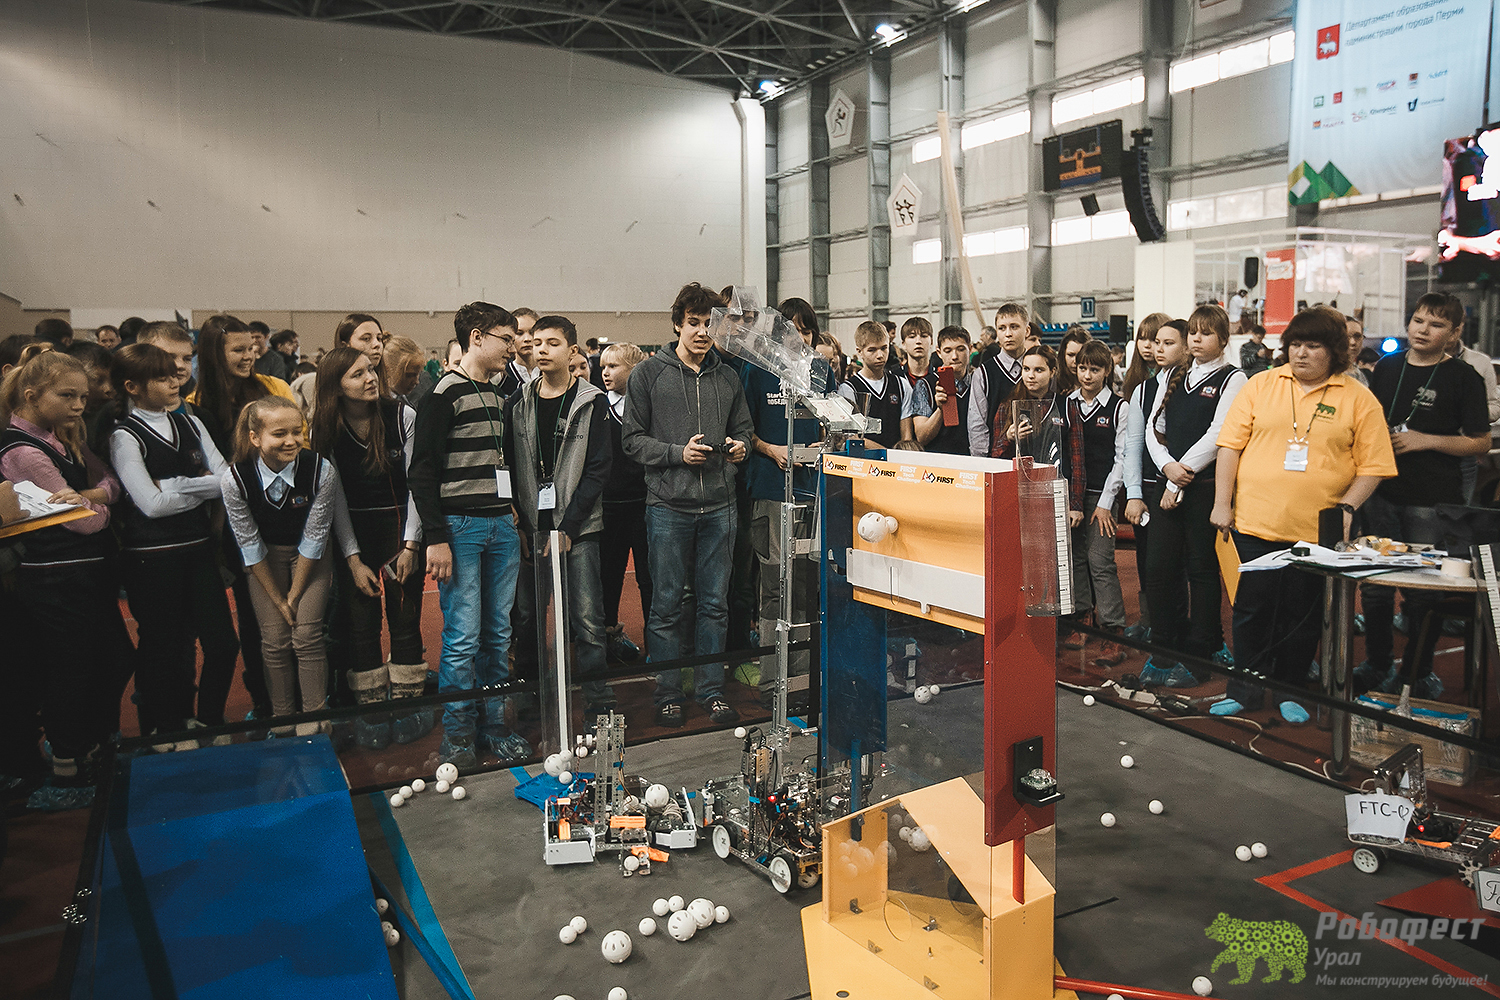
\includegraphics[scale=0.2]{days/Event/images/3}}\\
		\end{enumerate}  
	\subsubsection{Regional final}	
		This was the event, to which the team had been preparing for for six months. Approaching the competition with fully finished. At competitions communicated with all the teams that were there, discussing strategy and offering their help. During the competition statistics were conducted on all the teams, which helped in choosing allies for the final. Was also had an action plan for an alliance with any team. In the final, having received a the choice of allies, were chosen team with the most stable results, and the rate was at collaborative interaction of any pair of robots. Results: the alliance of winners as well as first place in the general classification, and the quota to World Championship.
			\center{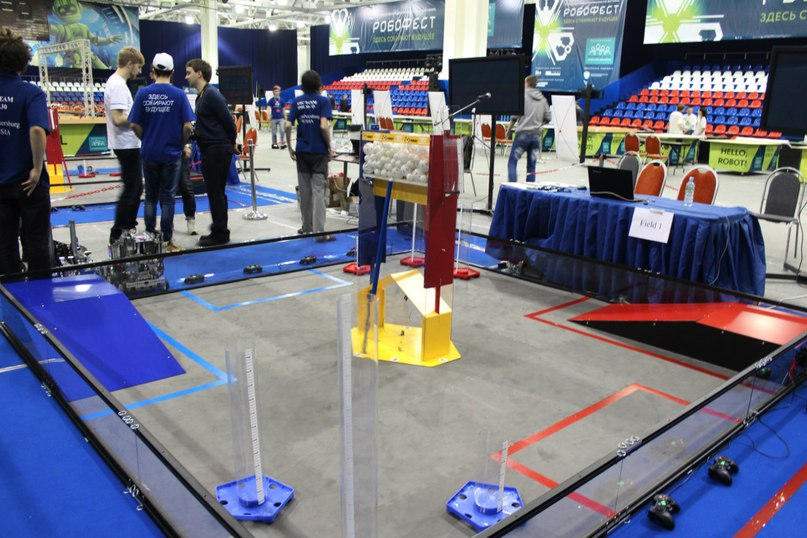
\includegraphics[scale=0.2]{days/Event/images/2}}\\
	\newpage			
	\subsubsection{CRDI RTC}
		Large Russian Institute of Robotics and Technical Cybernetics. A tour was organized for the team in the institute, where we could see the real processes of development of detailed design for robotics. There we saw several project summaries at different stages of development - from drawings to finished models, as well as commercially ready products. From there we learned some ways on how to organize. Internet adress http://www.rtc.ru.	\\
		\center{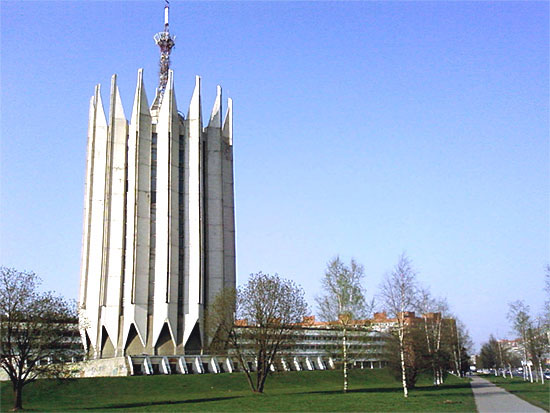
\includegraphics[scale=0.2]{days/Event/images/5}}\\
	\subsubsection{GeoScan}
		A Russian company thatproduces and sells unmanned aerial photography systems. There we were clearly shown how the office is designed, as well as the distribution of responsibilities and tasks, and what the internal interaction is like. Also, we were shown the whole production line. Internet adress http://geoscan.aero/.	
		\center{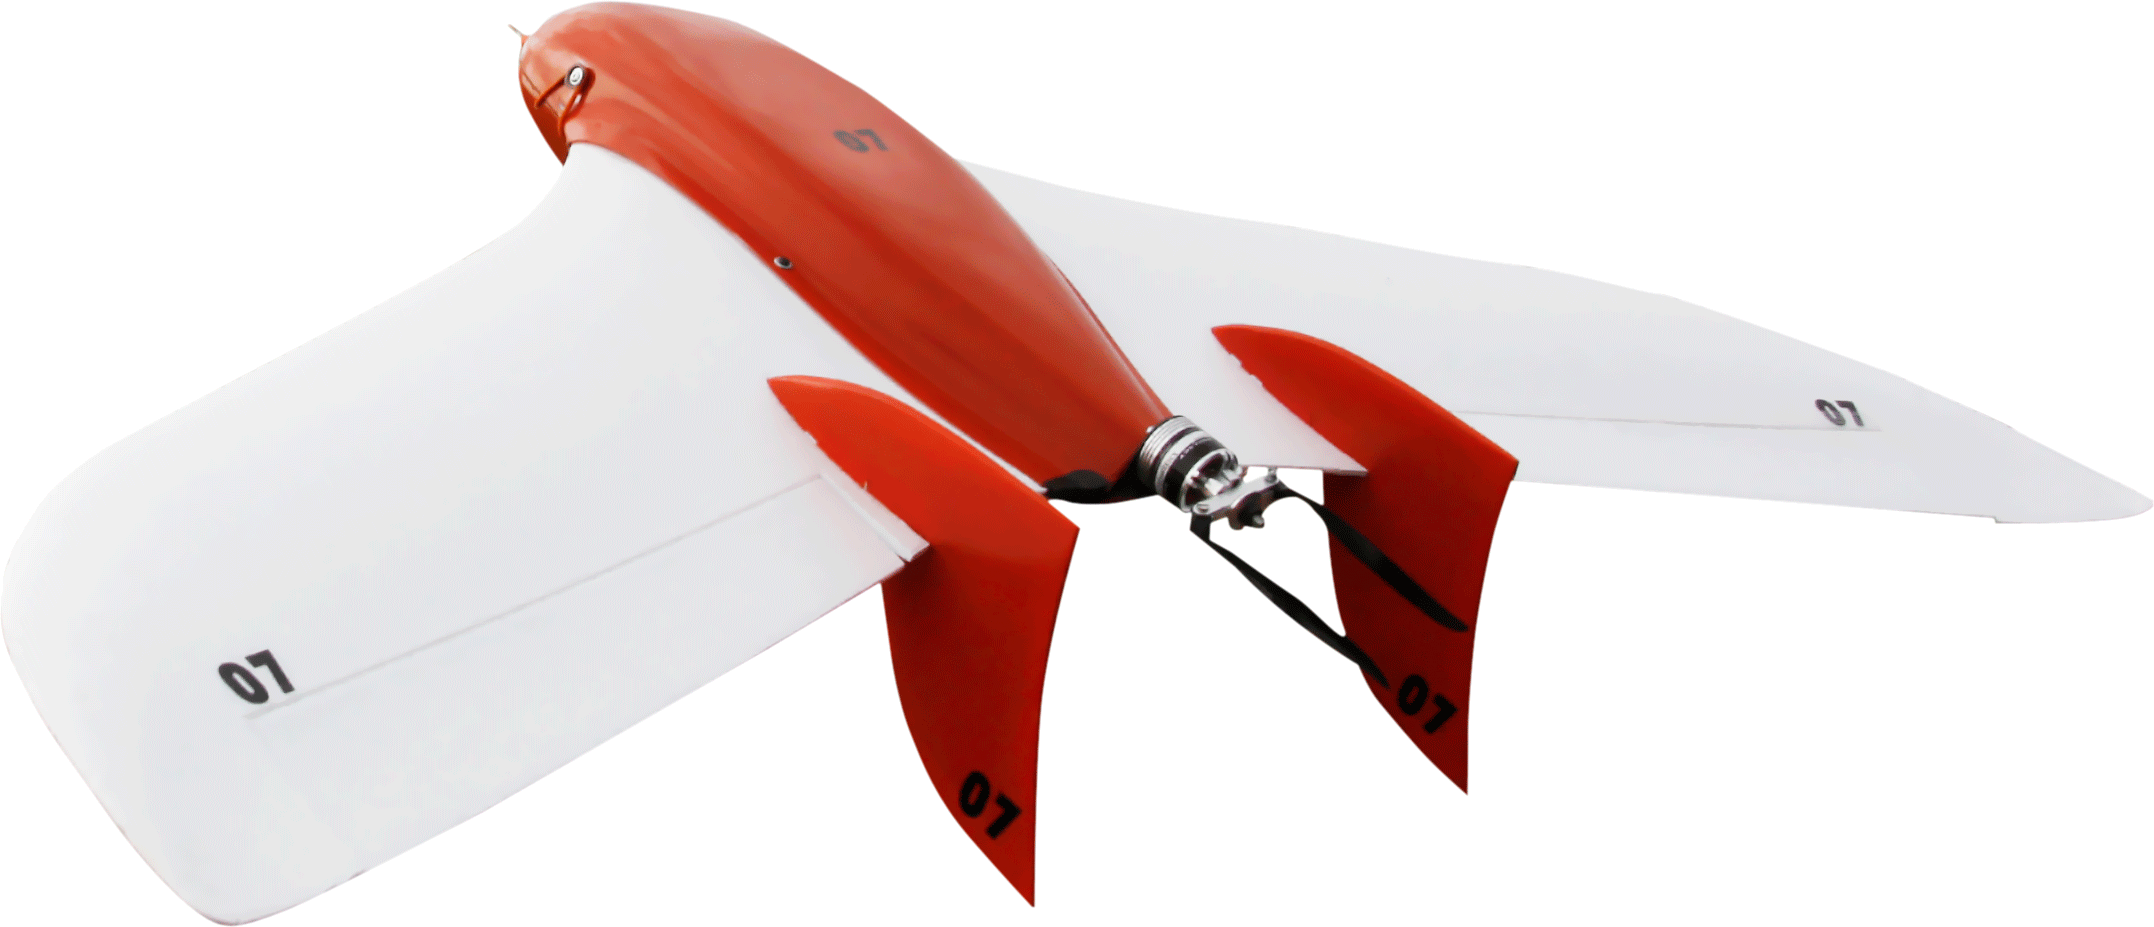
\includegraphics[scale=0.2]{days/Event/images/4}}\\
	\subsubsection{PML 30 landfill}	
		PML 30 landfill competitions are carried out by our organization. Their main  misrepresented that participant receives a rear and parts for its decision merely on the competition, compliance with the maximum being equal. We also demonstrated the FTC involving the participation.
		\center{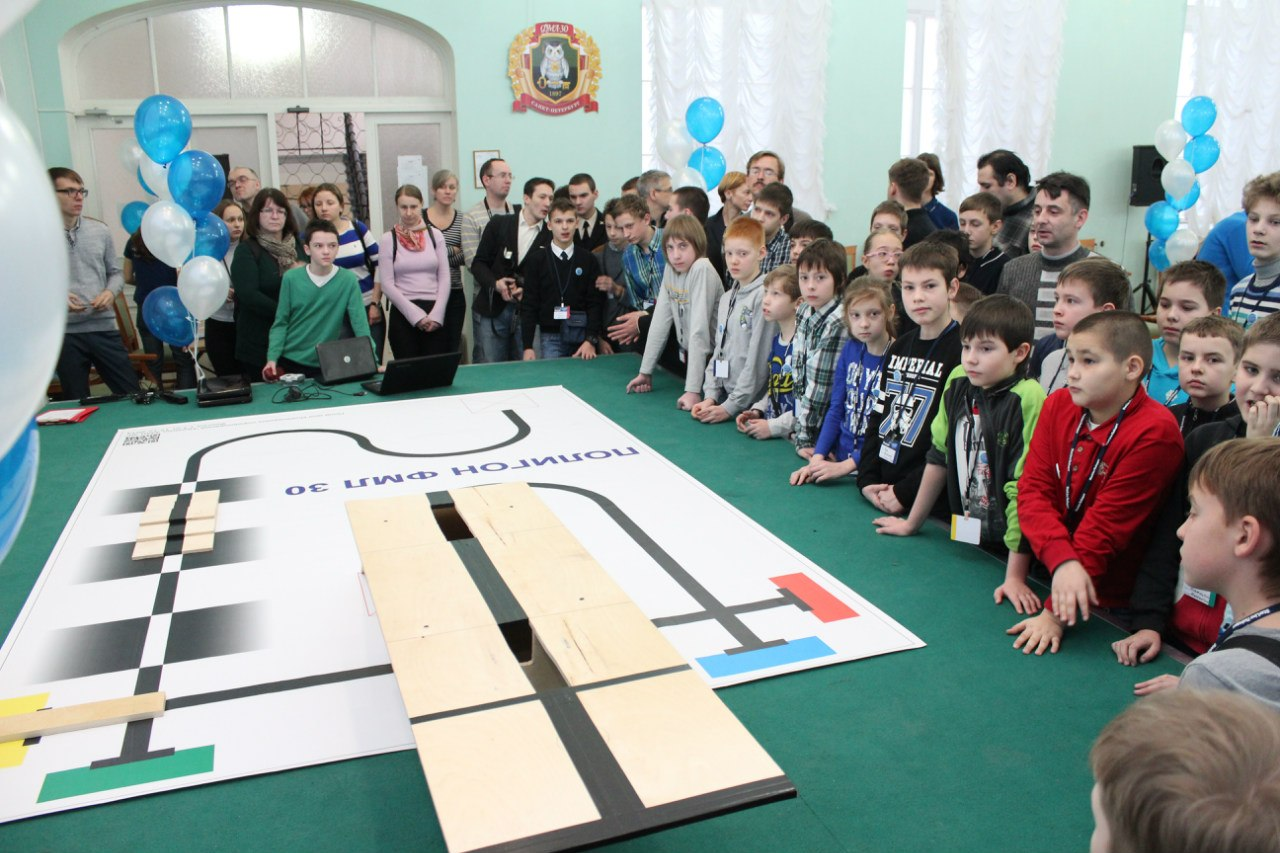
\includegraphics[scale=0.2]{days/Event/images/7}}\\
	\subsubsection{Summer camp on Robotics}
	In the camp in 2015, team members will conduct a robotics engineering course based on constructor TETRIX, attracting more people to the FTC.
		
		
		
		
		
		
		
		
		
